\documentclass{article}

\usepackage{mathpb} % custom mathematics package including AMSmaths/fonts

\usepackage{multicol}
\usepackage{psgo}
\usepackage{amsrefs}
\usepackage{subcaption}
\usepackage{hyperref}
\usepackage{graphicx}
\usepackage{float}
\usepackage{subfiles}

\theoremstyle{plain}
\newtheorem{theorem}{Theorem}[section]
\newtheorem{corollary}{Corollary}[theorem]
\newtheorem{lemma}{Lemma}[theorem]

\theoremstyle{definition}
\newtheorem{definition}{Definition}[section]

\hypersetup{linktoc=all}

\title{Solving One-Point Go Endgames with Combinatorial Game Theory}
\author{Anders Poirel - apoirel@ucsc.edu \\ University of California, Santa Cruz}
\date{Spring 2021}

\begin{document}

\maketitle

\begin{figure}[ht]
    \centering
    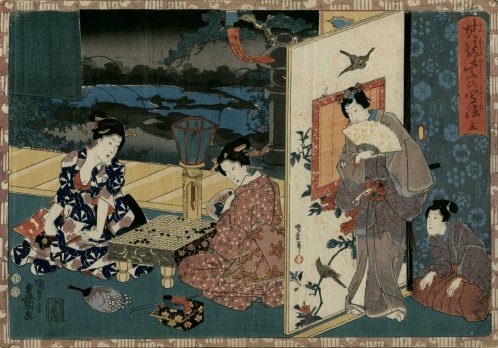
\includegraphics[width=\textwidth]{prince_genji.jpg}
\end{figure}

\begin{abstract}
    Combinatorial game theory studies deterministic, perfect-information 
    two-player games with guaranteed termination. Go is one of the canonical objects of study 
    in the field, and while the combinatorial complexity of the game is such that most positions cannot 
    be solved solved, many Go endgame positions can be decomposed into simpler objects which can be
    analyzed exactly using results from combinatorial game theory.
\end{abstract}

\newpage

Illustration: Toyokuni III, \textit{Prince Genji Watching Two Ladies Playing Go }, 
Izumiya Ichibei, 1849-1851.

\tableofcontents
\newpage 
\section{Introduction}

Go is known for its combinatorial complexity - a lower bound $10^{10^{48}}$ has 
been found on the number of possible Go games on a 19$\times$19 board \cite{senseilower}. 
Furthermore, during most of a Go game, stones on board are linked by
 subtle interdependencies which are not easily quantified. As such, it is in practice impossible 
to determine an optimal move at most stages of the game on any nontrivial board size (in fact, the 
largest board size to have been fully solved is $5\times5$).

However, using the tools from combinatorial game theory developed starting in the 1970s,
namely decomposition into independent position and chilling, exact results can be derived
for a restricted class of endgame Go problems, providing a decisive advantage over 
game tree search approaches.

By introducing illustrating the fundamental concepts of the theory immediately 
with Go positions, this paper attempts to convey how the theory naturally emerges from the rules 
of Go, despite being applicable to a much wider variety of two-player deterministic
games. 

\subfile{sections/game}

\section{Combinatorial Game Theory for Go}

\subfile{sections/game_theory}

\subfile{sections/simplifying_games}

\subfile{sections/surreal_numbers}

\section{One-point Go Endgames}

\subfile{sections/endgame}

\subfile{sections/temperature_theory}

\subfile{sections/positions_analysis}

\section{Conclusion}

\subfile{sections/conclusion}

\bibliography{references}

\end{document}